%
% File acl2020.tex
%
%% Based on the style files for ACL 2020, which were
%% Based on the style files for ACL 2018, NAACL 2018/19, which were
%% Based on the style files for ACL-2015, with some improvements
%%  taken from the NAACL-2016 style
%% Based on the style files for ACL-2014, which were, in turn,
%% based on ACL-2013, ACL-2012, ACL-2011, ACL-2010, ACL-IJCNLP-2009,
%% EACL-2009, IJCNLP-2008...
%% Based on the style files for EACL 2006 by 
%%e.agirre@ehu.es or Sergi.Balari@uab.es
%% and that of ACL 08 by Joakim Nivre and Noah Smith

\documentclass[11pt,a4paper]{article}
\usepackage[hyperref]{acl2020}
\usepackage{times}
\usepackage{latexsym}
\usepackage{graphicx}
\usepackage{url}
\renewcommand{\UrlFont}{\ttfamily\small}

% This is not strictly necessary, and may be commented out,
% but it will improve the layout of the manuscript,
% and will typically save some space.
\usepackage{microtype}

\aclfinalcopy % Uncomment this line for the final submission
%\def\aclpaperid{***} %  Enter the acl Paper ID here

%\setlength\titlebox{5cm}
% You can expand the titlebox if you need extra space
% to show all the authors. Please do not make the titlebox
% smaller than 5cm (the original size); we will check this
% in the camera-ready version and ask you to change it back.

\newcommand\BibTeX{B\textsc{ib}\TeX}

\title{The Dark Side of Language: Using NLP to Combat Hate Speech}

\author{ 
  Adam Hyman, 
  \texttt{adamhyman@berkeley.edu}
  \\[3ex]
  \textbf{Shalini Chawla, shalini\_chawla@berkeley.edu}
  \\[3ex]
  \textbf{Sreeram Ravinoothala, sreeram@berkeley.edu} 
  }

\date{April 2023}

\begin{document}
\maketitle
\begin{abstract}
With the advent of social media, people have had access to propagate hate anonymously, making it more dangerous than ever as the impact is not contained by a social group or geographic area any more. It is very important for social media companies to accurately identify hateful content and a lot of work has been already done to classify online content as toxic vs non-toxic for content moderation. We would like to extend this classification from binary to a a multi label classification and identify the specific hate categories toxic content belongs to. This information can be used by socio- political studies exploring the relationship between specific social-political events and their impact on triggering hateful content in online media. In this paper, we fine-tune three pre-trained large language models for a multi-label classification task to categorize text comments as toxic, severe\_toxic, obscene, threat, insult and identity\_hate. To tackle the imbalance of available training data, we use back translation using multiple intermediate to augment training data for the minority classes.

\end{abstract}

\section{Introduction}

In common language, “hate speech” refers to offensive discourse targeting a group or an individual based on inherent characteristics (such as race, religion or gender).

The adoption of social media brings in different views of many people. One of the primary issues bleeding the social media community is hate speech. Hate speech brings lot of negativity in people that if not curtailed can spiral into bigger issues like what we see around us in many cases. Hate speech can be targeted against individual, community, ideology etc. The social platforms with so many resources at hand are able to take care of it though much more is needed to cut it at the root.

With the advances in machine learning, many of the social media platforms have done a lot of great work in controlling the proliferation of hate speech by making use of classification algorithms but there is much more to be done to reduce the exposure to a great extent. They are successful in many ways but classifying the content to check if it indeed is hate is very complex as it depends on the context as well as whether its used loosely. There is lot of research done or going on classifying the text as well as augmenting such text.

The ability in building accurate models to correctly classify hateful content is a challenging task due to the limited availability of labeled data required for training. The training data needs to be labeled by human annotators. In addition to being a tedious task, it also exposes the annotators to the disturbing content in the data they are required to label. The public data sets available today are highly imbalanced and have very limited samples for some of the minority categories including threat, obscene and severe\_toxic compared to the large amount of non-toxic samples. We follow two approaches to deal with the limitations of data availability.

1) Pre-trained large language models have made it feasible to achieve better accuracy  in many NLP tasks where the amount of training data is limited, by providing word embeddings that have already learned characteristics of natural language. Using these pre-learned embeddings as the input to a classification model enables the model to learn to classify the content using much lesser amount of training data than it would have needed to learn the same relationship from scratch.

We use three large language models: BERT, T5 and XLNet and fine-tune them for a multi label classification task using our data set that has been labeled with the 6 toxicity classes. 

2) Our source data set is highly imbalanced and has very limited data for three out of the six categories. We use a combination of approaches to balance our data set to help the model balance learning across all categories. 
We have three minority categories: threat, severe-toxic and identity\_hate that have very low representation in our training data set. We use the TOXIGEN \cite{hartvigsen2022toxigen} data set to augment data for the identity\_hate class. To augment data for the other classes, we use back translation to generate additional samples from the existing data. 


\section{Background}
There has been a lot of research and previous work done with focus on toxic content  classification and a few different pathways have been explored to improve the accuracy of classification. 
The unavailability of enough quality labeled data has been widely accepted as a limitation in the ability to create accurate models for toxic content classification. \cite{rastogi2020can} has explored generating synthetic data using EDA and back translation to augment the training data and reported improved recall and F1 scores. \cite{hartvigsen2022toxigen} have explored the complexity of identifying implicit identity\_hate targeted at minority groups and used GPT-2 to generate additional data to augment the current available human labeled data sets. 
Another issue has been the inconsistency in labeling across the publicly available data sets limiting the generalization of trained models. 

\section{Data}

\subsection{Source Data Set}
We use the jigaw dataset from kaggle competition that was derived out of reddit data. The data set consist of 3 files that includes the labeled training data, test data and the test labels. We combine the test data and labels file by joining them on the unique comment identifiers. The training data set has 159,000 samples while the test data set has 60,000 samples. We convert the comments into lowercase and clean the contents by removing punctuation and special characters. Once processed both are training and test data file  consist of the text comments and binary labels for the 6 categories listed below.

\begin{itemize}
\item toxic
\item severe\_toxic
\item obscene
\item threat
\item insult
\item identity\_hate
\end{itemize}

\subsection{Data Balancing}
Our source data is highly imbalanced. Out of the 6 labeled classes, 3 are majority classes with and 3 are minority classes.
\begin{table}
\centering
\begin{tabular}{l r}
\hline
\textbf{Label} & \textbf{Count}\\
\hline
\verb|toxic| & 159000 \\
\verb|severe_toxic| & 1500 \\
\verb|obscene| & 500 \\ 
\verb|threat| & 500 \\ 
\verb|insult| & 500 \\
\verb|identity_hate| & 500 \\
\hline 
\end{tabular}
\caption{Distribution of toxicity labels in the source data set.}
\end{table}

\begin{figure}[h!]
\centering
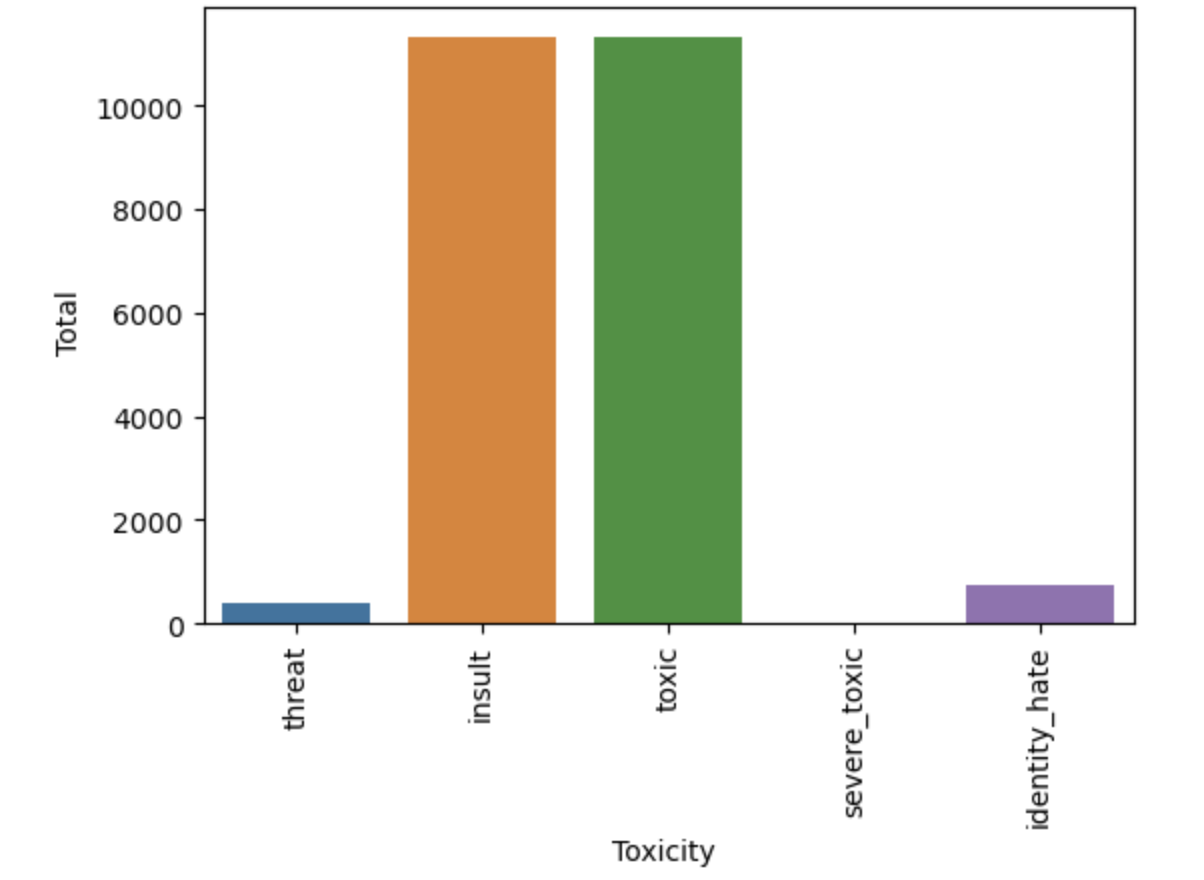
\includegraphics[width=50mm,scale=0.5]{label_counts.png}
\caption{Toxicity Label Count}
\label{Fig1. label count vs toxicity}
\end{figure}

\subsection{Undersampling Majority Class Data}
To balance the data set for the 6 classes being identified, we use a combination of strategies. We undersample two of two majority classes severe\_toxic and obscene to select 2000 random samples each from the original training data set. Since the label toxic is set to True if any of the 

\subsection{Augmenting Minority Class Data}
To bring the available training data for minority classes to be closer in count to the majority classes more balanced To augment the data for minority classes identity\_hate, we chose to augment with the data available from the TOXIGEN dataset[2]


\section{Methods}

\subsection{Baseline Model - BERT fine-tuned on source data}
Our baseline model is BERT base model(cased). We fine-tune the model on the full training data set that has been split into training and validation using 80:20 split and stratified on the 6 label classes. We add a hidden layer with 200 neurons and dropout layer with 0.3 before our final classification layer with 6 outputs to perform a multi label classification. We train the model for 2 epochs using learning rate of .00005 and batch size of 32.

The model performs really poorly for our 3 minority classes, completely failing to identify any of the severe\_toxic, threat and identity\_hate comments.

\begin{table}
\centering
\begin{tabular}{lrrr}
\hline
\textbf{class} & \textbf{prec} & \textbf{recall} & \textbf{f1-score}\\
\hline
\verb|toxic| & 0.62 & 0.40 & 0.49 \\
\verb|severe_toxic| & \textcolor{red}{0.00} & \textcolor{red}{0.00} & \textcolor{red}{0.00} \\
\verb|obscene| & 0.66 & 0.32 & 0.43 \\
\verb|threat| & \textcolor{red}{0.00} & \textcolor{red}{0.00} & \textcolor{red}{0.00} \\
\verb|insult| & 0.65 & 0.25 & 0.36 \\
\verb|identity_hate| & \textcolor{red}{0.00} & \textcolor{red}{0.00} & \textcolor{red}{0.00} \\
\vspace{2\baselineskip}\\
\verb|micro avg| & 0.64 & 0.31 & 0.42 \\
\verb|macro avg| & 0.32 & 0.16 & 0.21 \\
\verb|weighted avf| & 0.58 & 0.31 & 0.40 \\
\verb|samples avg| & 0.04 & 0.03 & 0.03 \\
\hline
\end{tabular}
\caption{Baseline Model - Classification Report}
\end{table}

\subsection{BERT fine-tuned with balanced data}
Our baseline model's poor performance is due to the much smaller amount of training data for the minority classes. To model is favoring the majority classes and is learning to just return the label as one of the majority classes to maximize accuracy since thats what most of the data is. To help our model learn the features of the minority classes, we create a new balanced data set by undersampling our majority classes and augmenting the minority classes. We run the BERT model with the same hyperparameters as in our baseline with the balanced data set.
Balancing the data set did not improve the classification score for minority classes at all it still stayed flat at 0 with none of the 3 minority classes being identified. Our data set size was reduced drastically after undersampling but we still had ~13,000 records which is an acceptable amount of data for fine-tuning BERT.
Since BERT was originally trained on wikipedia data and has not previously seen a majority of the vocabulary that is in the toxic data, it is not able to learn enough from the provided data to identify the minority classes. 


\subsection{Retraining BERT layers}
Our next step was to systematically unfreeze the pre-trained BERT layers 2 at a time and retrain them using our data set. We used the original unbalanced data set and the balanced dataset we created and re-trained the top 2 BERT layers, followed by 4, 6 and all the layers.
The first classifier with retraining only the top 2 BERT layers gave as a huge improvement in score for all three of the minority classes. As we retrained deeper layers, the total score kept moving upwards. For the full unbalanced dataset, the improvement stagnates after 4 layers. This has been observed in previous work done by \cite{Singh2020HowMD}. But we observed that with the smaller balanced dataset, the improvement continues as we retrain more layers with full retraining of all 12 layers giving us the best scores.


\subsection{T5}
We used T5-small \cite{raffel2020exploring} on the unbalanced training dataset similar to BERT. The model was adopted from \cite{t5mlcode}. As part of the multilabel classification a language modeling head is used on top of the decoder. The model was run 2 epochs with 8 and 16 batch size. The lesser epochs was because of the time the model was taking to train and predict. The model was very biased towards the higher dataset and also failed to predict the lower classes (insult, identity\_hate) which can be seen from the lower ROC-AUC scores.

The same experiment was repeated with balanced dataset for 2 epocks and 16 batch size. The results were similar to what was seen with unbalanced dataset. It was still not predicting the classes insult and identity\_hate properly.

With above results, it was not prudent for us to pursue with T5 due to no improvement in the metrics.

\subsection{XLNet}

\section{Results and Discussion}

Metrics were captured across multiple models that were tested as shown in Table ~\ref{table:UnBalResults} and Table ~\ref{table:BalResults}. Each model was run for multiple epochs to ensure proper outcome of metrics. Bert model was fine tuned by unfreezing different number of layers inorder for BERT to learn the toxic data. The data clearly shows how the model has improved with respect to F1 score as well as AUC-ROC numbers.

T5 was applied on unbalanced data and balanced data. But, the metrics are not too significantly different to say one of them is better.

Similarly XLNet model was applied on both unbalanced as well as balanced dataset.

There is a clear indication of how each model shines given a balanced dataset. XLNet clearly shows its predictions are way better than the other two models.

\begin{table*}
\centering
\begin{tabular}{lrrrrrrrrrr}
\hline
\textbf{Model} & \textbf{Macro} & \textbf{Macro} & \textbf{Toxic} & \textbf{Severe Toxic} & \textbf{Obscene} & \textbf{Threat} & \textbf{Insult} & \textbf{Id Hate}
\\
\textbf{ } & \textbf{F1} & \textbf{AUC} & \textbf{AUC} & \textbf{AUC} & \textbf{AUC} & \textbf{AUC} & \textbf{AUC} & \textbf{AUC}\\
\hline
\verb|BERT Baseline|&0.2&0.56& 0.66 & 0.5 & 0.63 & 0.5 & 0.61 & 0.5 \\
\verb|BERT 2-layers| & 0.5 & 0.74 & 0.88 & 0.6 & 0.87 & 0.57 & 0.8 \\
\verb|BERT 4-layers| & 0.55 & 0.78 & 0.9 & 0.59 & 0.86 & 0.71 & 0.88 & 0.72 \\
\verb|BERT 6-layers| & & & & & & & & \\
\verb|BERT 12-layers| & 0.49 & 0.77 & 0.9 & 0.73 & 0.89 & 0.49 & 0.88 & 0.73 \\
\verb|T5| & 0.07 & 0.59 & 0.53 & 0.94 & 0.51 & 0.58 & 0.5 & 0.5 \\
\verb|XLNet| & & & & & & & & \\
\hline
\end{tabular}
\caption{Metrics - All Models trained with original unbalanced data}
\label{table:UnBalResults}
\end{table*}

\begin{table*}
\centering
\begin{tabular}{lrrrrrrrrrr}
\hline
\textbf{Model} & \textbf{Macro} & \textbf{Macro} & \textbf{Toxic} & \textbf{Severe Toxic} & \textbf{Obscene} & \textbf{Threat} & \textbf{Insult} & \textbf{Id Hate}
\\
\textbf{ } & \textbf{F1} & \textbf{AUC} & \textbf{AUC} & \textbf{AUC} & \textbf{AUC} & \textbf{AUC} & \textbf{AUC} & \textbf{AUC}\\
\hline
\verb|Bert Baseline| & 0.05 & 0.51 & 0.57 & 0.5 & 0.5 & 0.49 & 0.5 & 0.5 \\
\verb|Bert 2 layers| & 0.42 & 0.86 & 0.85 & 0.79 & 0.87 & 0.91 & 0.83 & 0.89 \\
\verb|Bert 4 layers| & 0.44 & 0.87 & 0.6 & 0.88 & 0.87 & 0.92 & 0.83 & 0.88 \\
\verb|Bert 6 layers| & 0.5 & 0.83 & 0.87 & 0.73 & 0.83 & 0.88 & 0.79 & 0.9 \\
\verb|Bert 12 layers| & 0.51 & 0.89 & 0.89 & 0.87 & 0.88 & 0.9 & 0.87 & 0.91 \\
\verb|T5| & 0.12 & 0.61 & 0.77 & 0.92 & 0.52 & 0.49 & 0.5 & 0.5 \\
\verb|XLNet| & 0.42 & 0.89 & 0.89 & 0.83 & 0.89 & 0.95 & 0.88 & 0.92 \\
\hline
\end{tabular}
\caption{Metrics - All Models trained with augmented balanced data}
\label{table:BalResults}
\end{table*}

\section{Error Analysis}

\section{Conclusion}

%\section*{References}
%Rastogi, Chetanya, et al. “Can We Achieve More with Less? Exploring Data Augmentation for Toxic Comment Classification.” ArXiv:2007.00875 [Cs], 2 July 2020, arxiv.org/abs/2007.00875. Accessed 31 Mar. 2023.\\\\
%Thomas Hartvigsen, Saadia Gabriel, Hamid Palangi, Maarten Sap, Dipankar Ray, and Ece Kamar. 2022. ToxiGen: A Large-Scale Machine-Generated Dataset for Adversarial and Implicit Hate Speech Detection. In Proceedings of the 60th Annual Meeting of the Association for Computational Linguistics (Volume 1: Long Papers), pages 3309–3326, Dublin, Ireland. Association for Computational Linguistics.\\\\
%Toxic, Hateful, Offensive or Abusive? What Are We Really Classifying ... https://aclanthology.org/2020.lrec-1.838.pdf.\\\\
%Singh, Trisha, and Davide Giovanardi. How Much Does Pre-Trained Information Help? Partially Re-Initializing BERT during Fine-Tuning to Analyze the Contribution of Layers Stanford CS224N {Custom} Project.

\bibliographystyle{apalike}
\bibliography{acl2020}
\end{document}
